\documentclass[12pt]{article}
\usepackage[english]{babel}
\usepackage{lipsum}
\usepackage[square, numbers]{natbib}
\bibliographystyle{plainurl}
\usepackage{url}
\usepackage[utf8x]{inputenc}
\usepackage{amsmath}
\usepackage{graphicx}
\graphicspath{{images/}}
\usepackage{parskip}
\usepackage{fancyhdr}
\usepackage{vmargin}
\usepackage{hyperref}
\usepackage{todonotes}
\usepackage{textcomp}
\usepackage{float}
\usepackage{listings}
\usepackage{color} %red, green, blue, yellow, cyan, magenta, black, white
\definecolor{mygreen}{RGB}{28,172,0} % color values Red, Green, Blue
\definecolor{mylilas}{RGB}{170,55,241}
\setmarginsrb{2 cm}{2.5 cm}{2 cm}{2.5 cm}{1 cm}{1 cm}{1 cm}{1 cm}

\title{SPENVIS Report}
\author{M. Bergmann, A. Scharf}	
\date{\today}

\makeatletter
\let\thetitle\@title
\let\theauthor\@author
\let\thedate\@date
\makeatother

\pagestyle{fancy}
\fancyhf{}
\rhead{\theauthor}
\lhead{\thetitle}
\cfoot{\thepage}



\begin{document}

\lstset{language=Matlab,%
    %basicstyle=\color{red},
    breaklines=true,%
    morekeywords={matlab2tikz},
    keywordstyle=\color{blue},%
    morekeywords=[2]{1}, keywordstyle=[2]{\color{black}},
    identifierstyle=\color{black},%
    stringstyle=\color{mylilas},
    commentstyle=\color{mygreen},%
    showstringspaces=false,%without this there will be a symbol in the places where there is a space
    numbers=left,%
    numberstyle={\tiny \color{black}},% size of the numbers
    numbersep=9pt, % this defines how far the numbers are from the text
    emph=[1]{for,end,break},emphstyle=[1]\color{red}, %some words to emphasise
    %emph=[2]{word1,word2}, emphstyle=[2]{style},
}

%%%%%%%%%%%%%%%%%%%%%%%%%%%%%%%%%%%%%%%%%%%%%%%%%%%%%%%%%%%%%%%%%%%%%%%%%%%%%%%%%%%%%%%%%

\begin{titlepage}
	\centering
    \vspace*{0.5 cm}
    
\includegraphics[scale = 0.4]{images/lulea}\\[1.0 cm]

   	\vspace{2cm}
	\textsc{\Large Spacecraft Environment Interaction}\\[0.5 cm]

	\textsc{\large R7004R}\\[0.5 cm]	
	\rule{\linewidth}{0.2 mm} \\[0.4 cm]
	{ \huge \bfseries \thetitle}\\
	\rule{\linewidth}{0.2 mm}
	\\[0.5cm]
		\textsc{Analysis of the Cluster-II FM-8 (Tango) Mission}
		\\[2.5 cm]

	
	\emph{Authors:}\\
	Matthias Bergmann \\
	Arthur Scharf

	\vspace{2cm}
	
	{\large \thedate}\\[2 cm]
 
	\vfill
	
\end{titlepage}




%%%%%%%%%%%%%%%%%%%%%%%%%%%%%%%%%%%%%%%%%%%%%%%%%%%%%%%%%%%%%%%%%%%%%%%%%%%%%%%%%%%%%%%%%


\clearpage\thispagestyle{empty}\addtocounter{page}{-1} 
\abstract
\lipsum[1]

\pagebreak
%\section{Preface}
\tableofcontents
\thispagestyle{empty}
\addtocounter{page}{-1}
\pagebreak
\section{Introduction}
\lipsum[3]

%\section{Mission Definition}
\section{Mission Overview}

\subsection{Mission Definition}
The Cluster-II Mission is planned and executed by the European Space Agency and was launched on 16th of July 2016. The whole mission consists of four identical spacecrafts flying in a tetrahedral formation in a highly elliptical orbit, where each spacecraft is collecting various data on the space environment with its 11 scientific payload instruments. These in-situ measurements are done to build a very accurate 3D-Model of the earth's magnetosphere and thus to observe the magnetosphere interaction with the solar wind not only in a spatial but also in a temporal resolution.

The main goal of this mission is to examine and gather data especially on the plasma structures in the bow shock region, the magnetopause, polar cusps, the earth's magnetotail and the auroral zone, all of them regions with very interesting properties when it comes to the interaction with solar wind \citep{ESA:clusterWebsite}.

\begin{figure}[h]
	\centering
	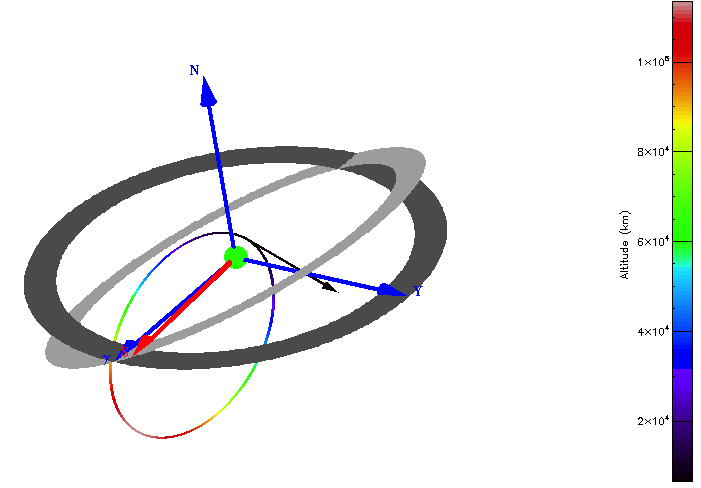
\includegraphics[width=\linewidth]{spenvis/3d_gei}
		\caption{One Orbit of FM-8 Tango, the color bar shows the altitude}
	\label{fig:orbit}
\end{figure}
To model the Orbit of FM-8 Tango a set of TLE (Two Line Element) data provided by CelesTrak was used \citep{celesTrak}.\\
Figure \ref{fig:orbit} shows one orbit of FM-8 Tango and indicates the altitude of the orbit. The orbit itself is a retrograde orbit with an inclination of 131.6 degrees. A complete set of TLE data describing all important orbit parameters can be found in the Appendix \ref{tleParameters}.




\subsection{Space Environment}

\subsection{Radiation Environment}


\section{Numerical Simulations}

\subsection{Environmental flux}

SPENVIS uses the AP-8/AE-8 model to simulate the trapped proton and electron models, which can simulate the fluxes during solar maximum and minimum.

For the worst-case simulation the solar maximum is considered. 

For the protons the number of trapped protons is higher during solar minimum due to the increased scale height caused by the increased UV radiation from the sun, but only for lower altitudes, for this orbit the difference between solar minimum and maximum for the proton flux is negligible, which is not the case for the electrons.

In figures \ref{fig:e_map} and \ref{fig:p_map} the integrated fluxes are displayed over the orbit in GEI mode.

The highes proton fluxes are expected at perigee, while for the electron flux the highes flux is expected during crossing of the radiation belts (c.f. fig. \ref{fig:e_wmap}).

\begin{figure}[!htbp]
  \centering
  \begin{minipage}[b]{0.45\textwidth}
    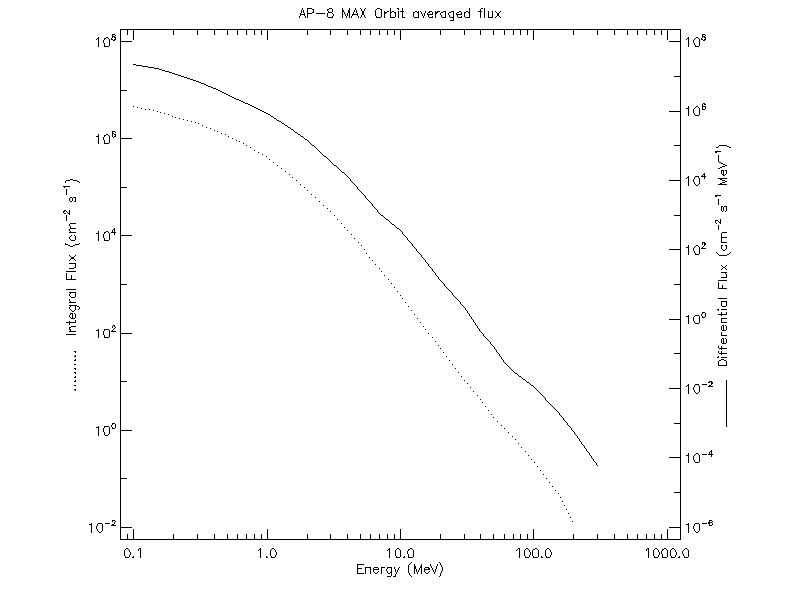
\includegraphics[width=\textwidth]{spenvis/max_prot}
    \caption{Proton Flux}
    \label{fig:p_flux}
  \end{minipage}
  \hfill
  \begin{minipage}[b]{0.45\textwidth}
    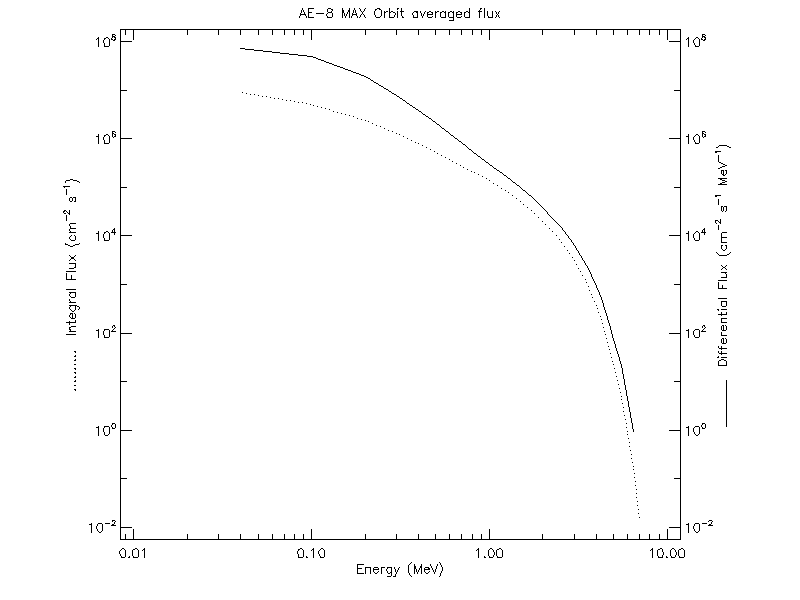
\includegraphics[width=\textwidth]{spenvis/max_elec}
    \caption{Electron Flux}
    \label{fig:e_flux}
  \end{minipage}
\end{figure}

\begin{figure}[!htbp]
  \centering
  \begin{minipage}[b]{0.45\textwidth}
    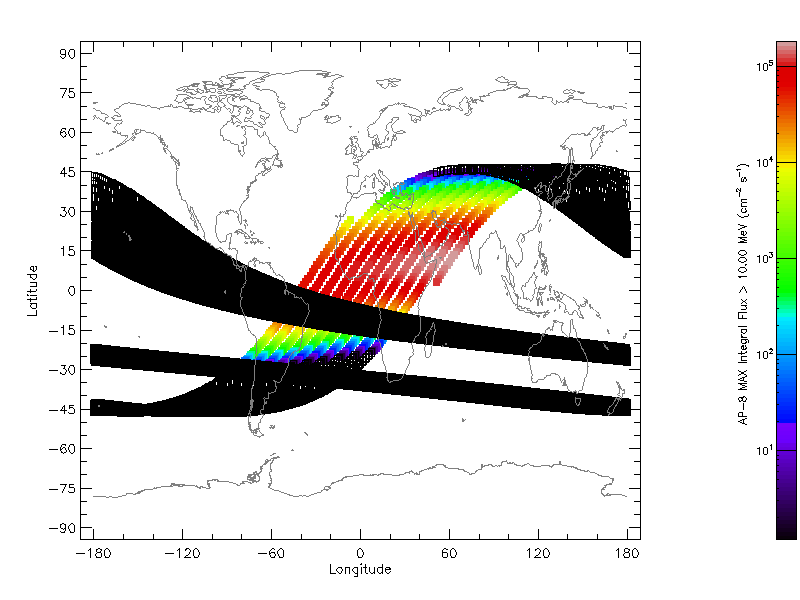
\includegraphics[width=\textwidth]{spenvis/proton_map}
    \caption{Proton Flux greater than 1 MeV}
    \label{fig:p_map}
  \end{minipage}
  \hfill
  \begin{minipage}[b]{0.45\textwidth}
    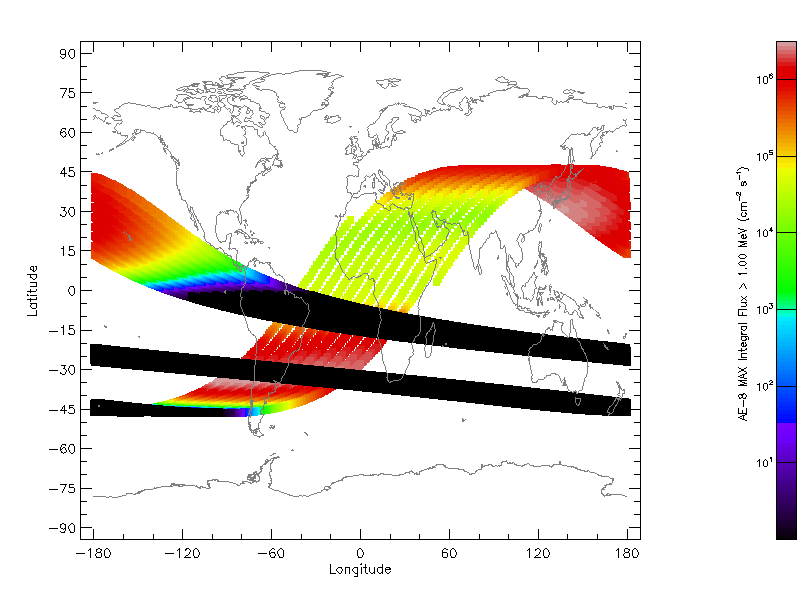
\includegraphics[width=\textwidth]{spenvis/electron_map}
    \caption{Electron Flux greater than 1 MeV}
    \label{fig:e_map}
  \end{minipage}
\end{figure}

\begin{figure}[!htbp]
	\centering
	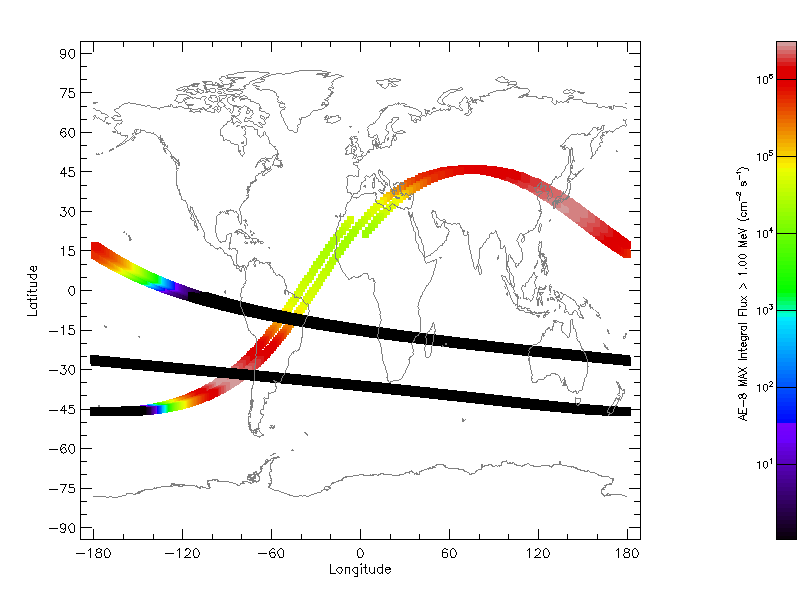
\includegraphics[width=.6\linewidth]{spenvis/electron_wmap}
		\caption{Electron Flux World map}
		 \label{fig:e_wmap}
\end{figure}

\subsection{Lifetime and Performance Degradation}

The satellite is using Azur 3G28 solar cells, with an EOL power of 95\% of the BOL power \citep{evans:labInstructions}.

Using SPENVIS' MC-SCREAM for solar cells, it was determined that the shielding thickness should be around 230 \textmu m which leaves an EOL powerloss of 3.3\%.

\subsection{Total Dose and Shielding}
\label{chap:dose}
The satellite is using a memory device which can withstand a total radiation dose of 25 Krad before failure.

With 1mm of shielding the memory device exceeds its maximum radiation dose with a total dose of 1.5 Mrad, which is about 62 times the maximum allowed dose.

To achieve a maximum dose of 25 Krad or less the shielding has to be increased to a minimum of 5.1mm, which will lead to a maximum dose of 26 Krad.

\begin{figure}[!htbp]
	\centering
	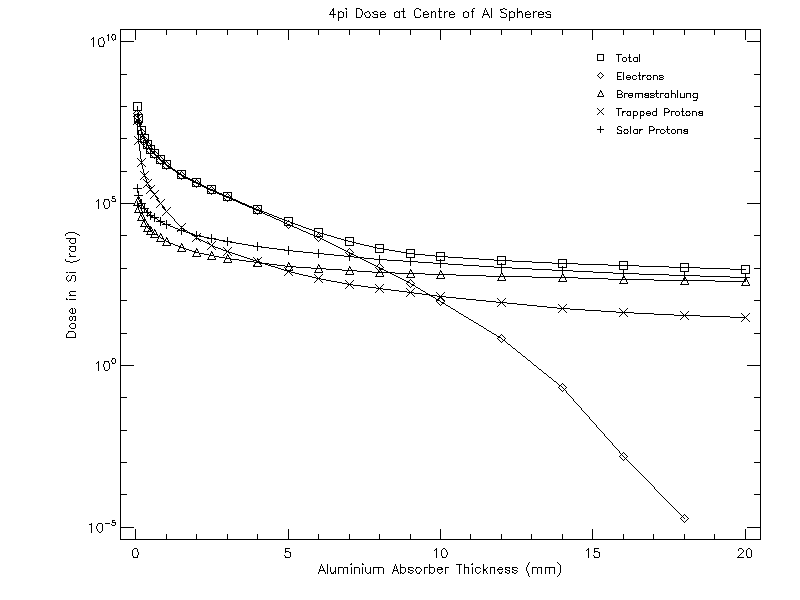
\includegraphics[width=.7\linewidth]{spenvis/memory_rad}
		\caption{Dose received vs. Shielding in mm}
		 \label{fig:rad_memory}
\end{figure}


\subsection{Single Event Upsets}

\subsubsection{Linear Energy Transfer (LET) Spectrum}

The LET spectra was calculated using SPENVIS, including solar particles, trapped protons and galactic cosmic rays, with a shielding of 1 $g/cm^2$ (c.f. fig. \ref{fig:let_spectra}).

\begin{figure}[H]
	\centering
	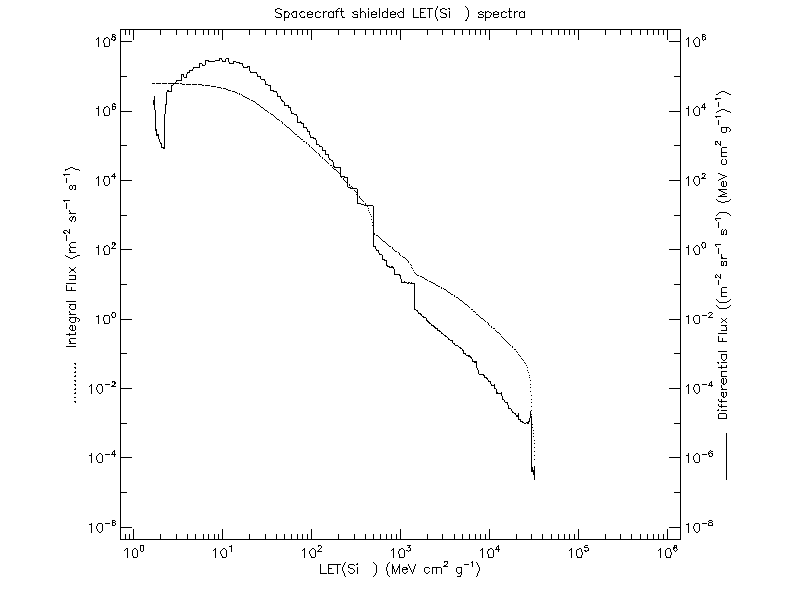
\includegraphics[width=.7\linewidth]{spenvis/LET_spectra}
		\caption{LET spectra for the full mission}
		 \label{fig:let_spectra}
\end{figure}

\subsubsection{Cross Section and Components Characteristics}

For the SEU estimation several parameters are needed for the SMJ329C50GFAM66 to determine its cross-section which is determined by a Weibull function, since only experimental data for the device are available \citep[Table 4]{evans:labInstructions}.

\begin{equation*}
\sigma(L) = \begin{cases}
0 &\text{$L \geq L_0$}\\
C_s \left ( 1 - e^{\left (\frac{L-L_0}{W}  \right )^{s} } \right ) &\text{$L < L_0$}
\end{cases}
\label{eqn:weibull}
\end{equation*}

Using the mono-beam experimental results (\citep{evans:labInstructions}) the final parameters calculated with a Weibull-fit in Matlab are:
\begin{table}[!htp]
 \centering
 \begin{tabular}{lcr}
  $L_0$ & $1.01 MeV\cdot cm² / mg$  & LET Threshold\\
  $C_s$ & $4.985 10^{-6} cm²$  & saturated crosssection\\
  $W$ & $4.985 MeV\cdot cm² / mg$  & Weight of the distribution\\
  $s$ & $0.7$  & shape parameter\\
 \end{tabular}
 \label{table:weibull}
 \caption{Results of the Weibull-Fit}
 \end{table}
 
 The code responsible for the fit is generated using the Matlab Curve-Fit Toolbox (c.f. Listing \ref{code:fit}) using data from \citep{evans:labInstructions} (c.f. Listing \ref{code:fit_values}), the graphical result of the fit is shown in figure \ref{fig:fit}.
 
 \begin{center}
\begin{lstlisting}[language=Matlab,caption={Autogenerated Matlabcode for fitting},label=code:fit]

function [fitresult, gof] = createFit(stopping, crossSec)
%CREATEFIT(STOPPING,CROSSSEC)
%  Create a fit.
%
%  Data for 'Weibull' fit:
%      X Input : stopping
%      Y Output: crossSec
%  Output:
%      fitresult : a fit object representing the fit.
%      gof : structure with goodness-of fit info.
%
%  See also FIT, CFIT, SFIT.

%  Auto-generated by MATLAB on 27-Mar-2016 22:16:28

[xData, yData] = prepareCurveData( stopping, crossSec );

% Set up fittype and options.
ft = fittype( 'C*(1-exp(-((x-L)/w)^s))', 'independent', 'x', 'dependent', 'y' );
opts = fitoptions( 'Method', 'NonlinearLeastSquares' );
opts.Display = 'Off';
opts.StartPoint = [0.0003 1 1 2];

% Fit model to data.
[fitresult, gof] = fit( xData, yData, ft, opts );
\end{lstlisting} 
 \end{center} 


 \begin{center}
\begin{lstlisting}[language=Matlab,caption={Inputvalues for the fit},label=code:fit_values]
flips =[8 7497 22514 23986 33810 29991 21022 18043]; %from instructions
exTime = [5 5 5 5 5 10 10 15]; %from instructions
flux = [25e6 25e6 25e6 17e6 23e6 10e6 7e6 4e6]; %from instructions
energyBeam = [0.6 0.72 9.6 4.8 20 56 84 786]; %from instructions
u = [12 12 12 16 40 56 84 131]; %from instructions
energy = energyBeam./(u); %Where it has to be read from the table
crossSec=flips./(exTime.*60.*flux); %crosssection
LET = [2.73E+03 3.13E+03 4.65E+03 7.23E+03 1.77E+04 2.77E+04 3.74E+04 5.72E+04]./1000; %MEV cm^2/mg, read from table
\end{lstlisting} 
 \end{center} 
 
 \begin{figure}[!htbp]
	\centering
	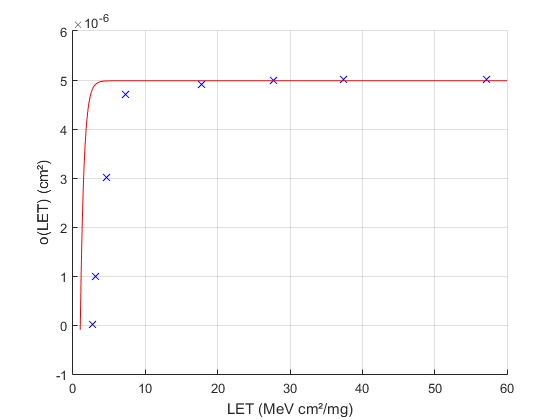
\includegraphics[width=.7\linewidth]{spenvis/fit}
		\caption{Weibull fit result}
		 \label{fig:fit}
\end{figure}

\subsubsection{SEU Estimation}

To determine which device is best for the mission it is neccessary which possible device is most immune to radiation to minimize malicious operation or data corruption.

This is done by estimating the SEU (single-event upset).

The SEU is calculated with the following formula (assuming omnidirectional flux), which was done using the results from the SPENVIS simulation in Matlab.

\begin{equation*}
\frac{dU}{dt} = 4 \pi \int_{0}^{\infty} \sigma\left ( LET \right ) \sum_{z=92}^{z=0}h\left ( LET \right )dLET
\end{equation*}

The resulting SEU in \( \frac{1}{sec} \) are

\begin{table}[!htp]
 \centering
  \caption{SEU rates}
 \begin{tabular}{lcr}
  NMOS2164 & $9.6 \cdot 10^{-3}$\\
CMOS R160-25 & $2.5 \cdot 10^{-6}$\\
Bipolar 93L422 & $13.8 \cdot 10^{-3}$\\
   SMJ329C50GFAM66 & $3.0 \cdot 10^{-3}$\\
 \end{tabular}
 \label{table:seu_rate}

 \end{table}
 
 As one can see easily in table \ref{table:seu_rate} the CMOS R160 has the lowest SEU rates of all devices, thus it is the best choice. The differential Flux is plotted against the LET for the four devices in Fig. \ref{fig:seu}.
 
  \begin{figure}[H]
	\centering
	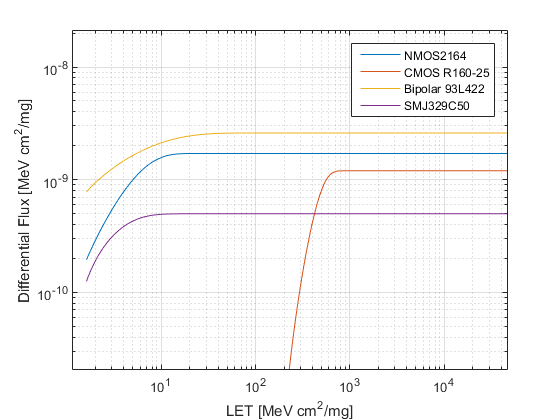
\includegraphics[width=\linewidth]{spenvis/seu}
		\caption{Plot of different LETs}
		 \label{fig:seu}
\end{figure}
\section{Conclusion}
In this report we analysed the Cluster-II FM-8 Tango Mission by the European Space Agency with regard to the space environment the satellite is in during its lifetime.

The first chapter introduced the mission of FM-8 Tango, where four similar satellites are building a very accurate 3D-Model of the earth's magnetosphere to analyse and understand its regions better, and described the orbit and its different effects it has on the spacecraft, as drag, erosion and radiation effects.

Having defined these constraints, we modelled the mission with the tool SPENVIS, to run simulations on the spaceraft environment, especially with focus on the radiation effects it has on the spacecraft.
Due to the degradation of the Azur 3G28 solar cells, which we assumed to be used on the spacecraft, as stated in the report instructions, we found out that the shielding thickness for the mission time should be 230 $\mu$m to reduce the incoming flux to have an acceptable degradation at the EOL.

In addition, we analysed the total ionising dose on a memory device to determine the necessary shielding to achieve a maximum dose of 25Krad on the device, which we found out to be minimum 5.2mm.

Since Drag Forces and Atomic Oxygen Effects were very small, they were neglected for further calculations \citep{vallado2008}.

Also, since the plasma environment affects the spacecraft in terms of spacecraft charging amongst other effects, we analysed the LET Spectra, including solar particles, trapped protons and GCR's with the help of SPENVIS and determined the cross section and component characteristics for four different memory devices, which were needed for the SEU estimation.
Having only experimental data on one of the devices, we applied curve fitting techniques to finally calculate the SEU rate for all devices.

Comparing the results of SEU rates, we were able to pinpoint the CMOS R160-25 device as the most suitable device for the FM-8 Mission, since it has the least amount of Single Event Upsets with $2.5 \cdot 10^{-6}$  \( \frac{1}{sec} \), compared to the other three devices.




\newpage
\phantomsection
\addcontentsline{toc}{section}{References}
\bibliographystyle{plain}
\bibliography{biblist}

\newpage
\phantomsection
\addcontentsline{toc}{section}{Appendix}
\section*{Appendix}

\subsection*{Orbital Parameters of Cluster-II FM8 Tango}
\label{tleParameters}
\texttt{CLUSTER II-FM8 (TANGO)\\
1 26464U 00045B 16087.81656212 .00000382 00000-0 00000+0 0 9996\\
2 26464 131.5572 328.3783 5181518 141.3516 0.4910 0.44219885 51441}

\vspace{1em}
%Table \ref{table:tle} shows the parameters extracted from the TLE data in a more readable format.

\begin{table}[h!]
\centering
\caption{Cluster-II Tango Parameters extracted of TLE set}
\label{table:tle}
\begin{tabular}{|c | c|} 
 \hline
 \textbf{Parameter} & \textbf{Value} \\ [0.5ex] 
 \hline
 Satellite Common Name &  CLUSTER II-FM8 TANGO\\ 
 Satellite Number &  26464\\
 Elset Classification &  U\\
 International Designator &  00\\
 Launch Number of the Year & 045\\
 Epoch Year & 16\\
 Epoch & 87.81656212\\
 BSTAR Drag Term &  0.00000382\\
 Inclination (deg) &  131.5572\\
 RAAN (deg) &  328.3782\\
 Eccentricity &  0.5181518\\
 Argument of Perigee (deg) &  141.3516\\
 Mean Anomaly (deg) &  0.4910\\
 Mean Motion (rev/day) &  0.44219885\\
 Rev number at epoch &  5144 \\ [1ex] 
 \hline
\end{tabular}
\end{table}


%%%%%%%%%%%%%%%%%%%%%%%%%%%%%%%%%%%%%%%%%%%%%%%%%%%%%%%%%%%%%%%%%%%%%%%%%%%%%%%%%%%%%%%%%



\end{document}